\documentclass[ignorenonframetext,t]{beamer}
\usetheme{Pittsburgh}
\setbeamertemplate{footline}[frame number]
\setbeamertemplate{bibliography item}[text]
\setbeamertemplate{navigation symbols}{}
\usepackage{pstricks}
\usepackage{pst-node}
\usepackage{pst-func}
\usepackage{pst-dbicons}

\setbeamercolor{codeexample}{fg=black,bg=blue!10}
\newcommand{\code}[1]{
\begin{beamercolorbox}[wd=\textwidth,rounded=true,shadow=true]{codeexample}
#1
\end{beamercolorbox}
}

\setbeamercolor{outputexample}{fg=white,bg=black}
\newcommand{\cmdoutput}[1]{
\begin{beamercolorbox}[wd=\textwidth,rounded=true,shadow=true]{outputexample}
#1
\end{beamercolorbox}
}

\title{iOS as a Scratch gamepad}
\author[M. Bateman]{Martin Bateman}
\date{5th August 2013}

\begin{document}

\frame{
\maketitle
}

%\begin{frame}{Scratcher Control}
%\begin{itemize}
%	\item Allows you to control Scratch from an Android phone\cite{scratchercontrol}
%\end{itemize}
%\begin{figure}[ht!]
%	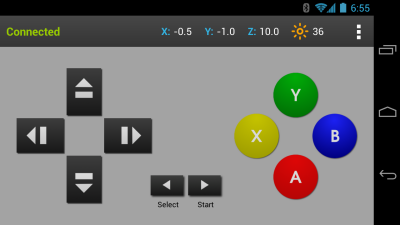
\includegraphics[scale=0.5]{images/scratchercontrol_screen.png}
%\end{figure}
%\begin{itemize}
%	\item Android only, many school have iOS
%\end{itemize}
%\end{frame}

\begin{frame}{Scratch Controllers}
\begin{itemize}
	\item Cat Wii Pi\cite{catwiipi} - Using a Wii controller with Scratch
	\item Scratcher Control\cite{scratchercontrol} - Control Scratch from an Android phone
\end{itemize}
\end{frame}

\begin{frame}{Scratch Control}
\begin{itemize}
	\item Requirement is iOS based
	\begin{itemize}
		\item due to school deployment
	\end{itemize}
	\item Would be good if
	\begin{itemize}
		\item easy deployment
		\item works with multiple phones (not just iOS)
		\item redefinable
	\end{itemize}
	\bigskip
	\item Go HTML5 based
	\begin{itemize}
		\item easily deployable
		\begin{itemize}
			\item any modern phone
		\end{itemize}
	\end{itemize}
\end{itemize}
\end{frame}

\begin{frame}{Architecture}
\begin{figure}
\begin{pspicture}(10,6)
\psframe(0,4)(2,6)
\rput[c](1,5.25){HTML5}
\rput[c](1,4.75){Browser}


\psframe(4,4)(6,6)
\rput[c](5,5){Proxy}

\psframe(8,4)(10,6)
\rput[c](9,5){Scratch}

\only<2->{
	\psline[arrowsize=0.2cm 2,arrowlength=1.4,arrowinset=0.4]{->}(2,5.75)(4,5.75)
	\rput[l](0.2,2.5){1) Get web page}
}

\only<3->{
	\psline[arrowsize=0.2cm 2,arrowlength=1.4,arrowinset=0.4]{<-}(2,5.5)(4,5.5)
	\rput[l](0.2,2){2) Return default page}
}

\only<4->{
	\psline[arrowsize=0.2cm 2,arrowlength=1.4,arrowinset=0.4]{->}(2,5.25)(4,5.25)
	\rput[l](0.2,1.5){3) Request controller}
}

\only<5->{
	\psline[arrowsize=0.2cm 2,arrowlength=1.4,arrowinset=0.4]{<-}(2,5)(4,5)
	\rput[l](0.2,1){4) Return controller}
}

\only<6->{
	\rput(3,4.75){JSON}
	\psline[linecolor=red,arrowsize=0.2cm 2,arrowlength=1.4,arrowinset=0.4]{->}(2,4.5)(4,4.5)
	\rput[l](0.2,0.5){5) Socket connection}
	\rput[l](0.6,0){5.1) browser to Proxy uses WebSocket}
	\rput[l](0.6,-0.5){5.2) Proxy to Scratch uses Remote Sensor}

	\psline[linecolor=red,arrowsize=0.2cm 2,arrowlength=1.4,arrowinset=0.4]{->}(6,4.5)(8,4.5)
	\rput(7,5.7){Scratch}
	\rput(7,5.25){Remote} 
	\rput(7,4.8){Sensor}
}

\only<3>{
	\rput[l](5,2){
		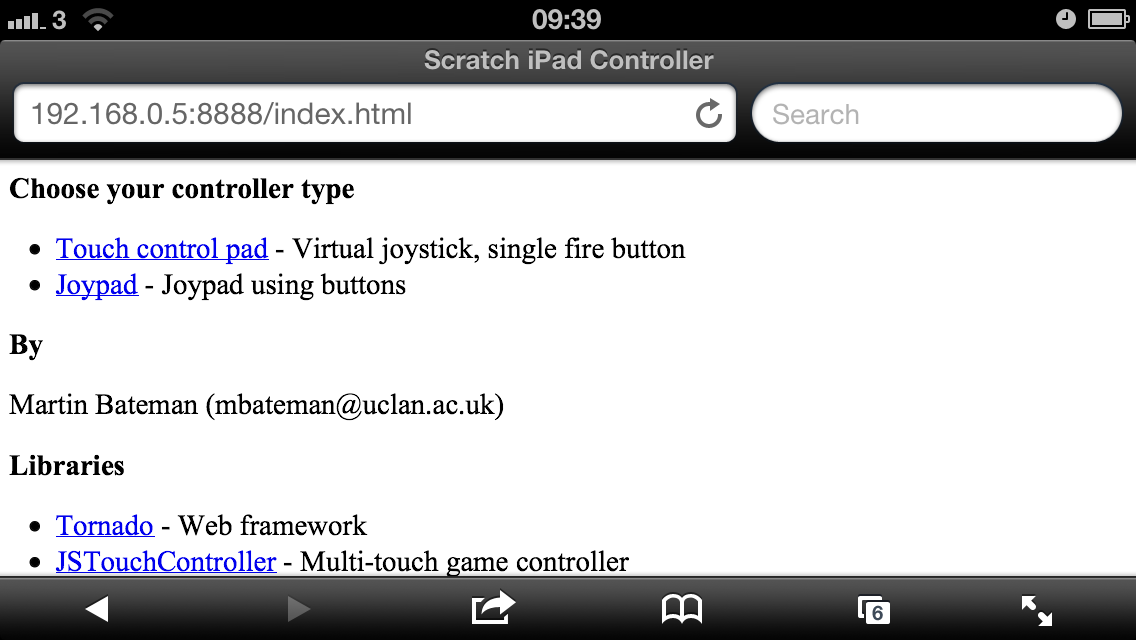
\includegraphics[scale=0.15]{images/default.png}
	}
}

\only<5->{
	\rput[l](5,2){
		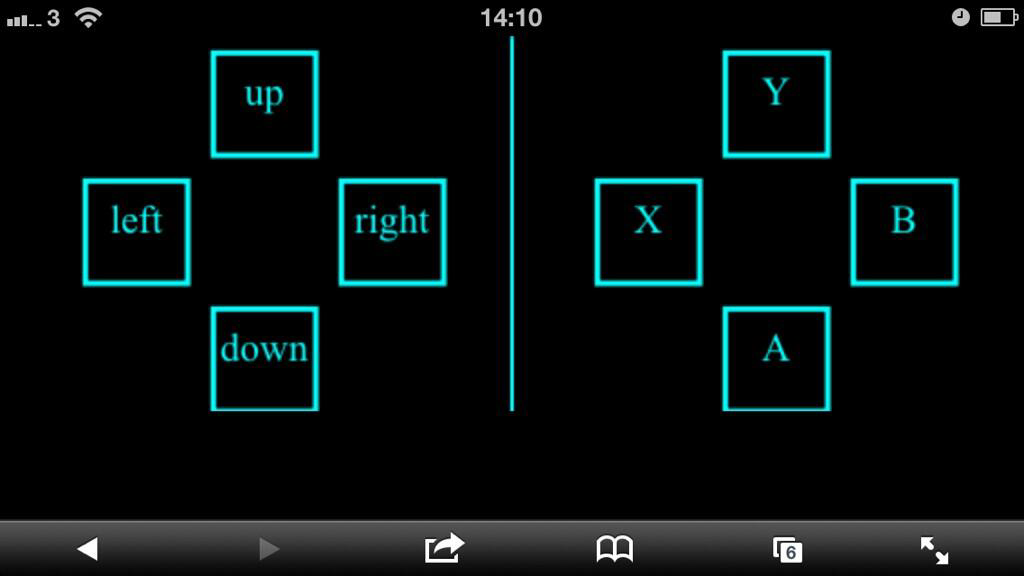
\includegraphics[scale=0.15]{images/touchpad.png}
	}
}

\end{pspicture}
\end{figure}
\end{frame}

\begin{frame}{Touchpad controller}
\begin{itemize}
	\item Joypad interface
	\item Each button sends a broadcast during interaction
	\begin{itemize}
		\item broadcasts being touched (eg 'left')
		\item broadcasts when no longer begin touched (eg 'released-left')
	\end{itemize}
\end{itemize}
\begin{figure}
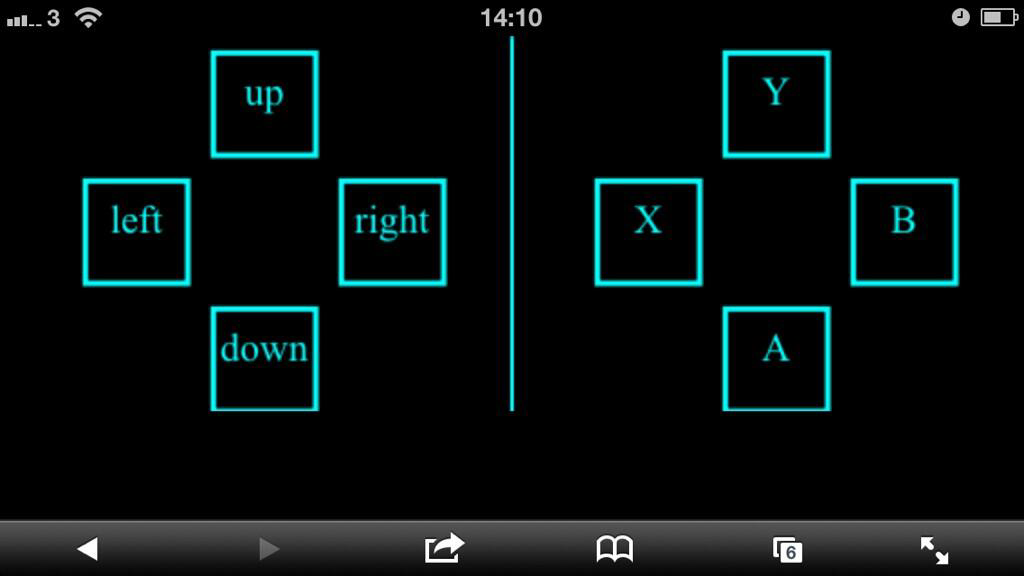
\includegraphics[scale=0.2]{images/touchpad.png}
\end{figure}
\end{frame}

\begin{frame}{Device orientation}
\begin{pspicture}(10,8)
\rput(5,4){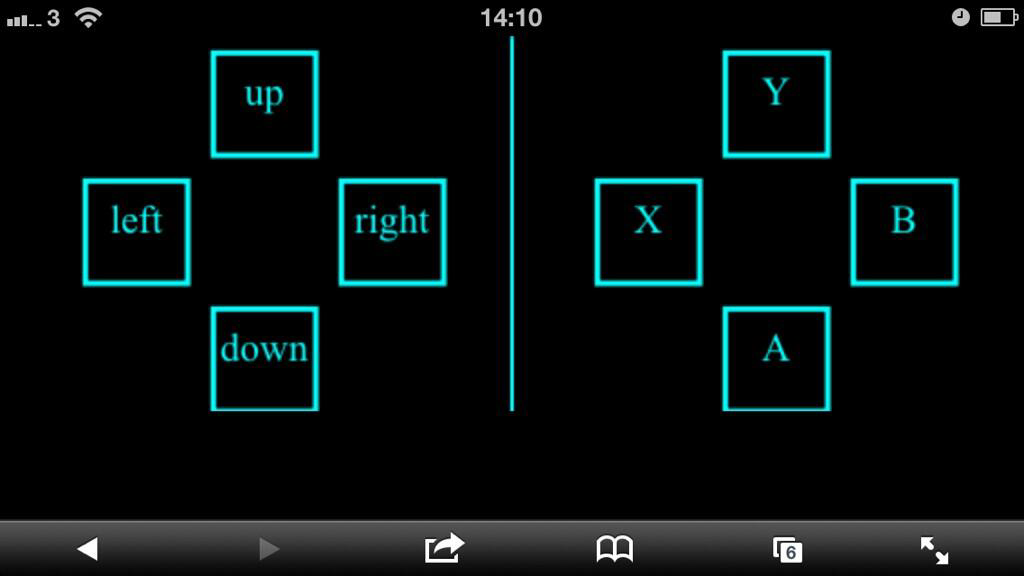
\includegraphics[scale=0.2]{images/touchpad.png}}

\only<1>{
\pscurve[linecolor=red,arrowsize=0.2cm 2,arrowlength=1.4,arrowinset=0.4]{<->}(1.5,6.5)(5,7.5)(8.5,6.5)
\rput(5,8){Turn}
}

\only<2>{
\pscurve[linecolor=red,arrowsize=0.2cm 2,arrowlength=1.4,arrowinset=0.4]{<-}(3.8,5)(5,7.5)(6, 6.05)
\rput(5,8){Tilt}
}
\only<3>{
\psline[arrowsize=0.2cm 2,arrowlength=1.4,arrowinset=0.4]{<->}(5, 7.5)(5, 6.5)
\psline[arrowsize=0.2cm 2,arrowlength=1.4,arrowinset=0.4]{<->}(4.5, 7)(5.5, 7)

\psline{<->}(4.75, 6.75)(5.25, 7.25)
\psline{<->}(4.75, 7.25)(5.25, 6.75)

\rput(5,7.65){\small{N}}
\rput(5,6.35){\small{S}}

\rput(4.35, 7){\small{W}}
\rput(5.65, 7){\small{E}}

\rput(5,8){Compass}
}

\end{pspicture}
\end{frame}

%\begin{frame}{Editing the UI}
%\begin{itemize}
%	\item Buttons are defined in a 2D array
%	\item Each entry looks like
%	\begin{itemize}
%		\item $<$x$>$, $<$y$>$, $<$width$>$, $<$height$>$, $<$name$>$
%	\end{itemize}
%\end{itemize}
%\end{frame}

\begin{frame}{References}
\bibliographystyle{IEEEtran.bst}
\bibliography{references.bib}
\end{frame}

\end{document}

